L'electrònica s'encarrega de rebre i processar el senyal elèctric emès pel fotosensor i emmagatzemar la informació pertinent. La diferents tasques realitzades per l'eslectrónica són aplicar humbrals energétics sobre la senyal (utilitzats per descartar senyals no perteneixents a esdeveniments de triti), amplificar la senyal (per tindre millor presició en les operacions realitzades sobre esta) y aplicar coincidencies temporals (per reduir la quantitat d'esdeveniments no perteneixents al triti). Finalment es realitza un histograma dels senyals que han superat totes les estacions anteriors, obtenint un espectre amb l'informació d'interes (l'energía dels esdeveniments). 

L'electrónica depén del tipus de senyal que reb i, per tant, depèn del tipus de fotosensor utilitzar. Degún a açò, en la col·laboració TRITIUM se empleen electróniques diferents, una per a les matrius de SiPMs i altra per a els PMTs:

\begin{itemize}

\item{} L'electrónica empleada per a cuan s'utilitzen matrius de SiPMs s'anomena PETsys \cite{PETSYS}, mostrat a la Figura \ref{fig:PETSYSs}, un sistema comercial desarrollat específicament per a treballar amb matrius de SiPMs. 

\begin{figure}[h]
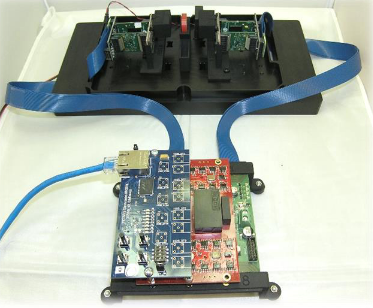
\includegraphics[scale=0.5]{12Summary/3DesignPrinciples/32Tritium_detector/PETSYS_System.png}
\centering
\caption{Sistema comercial PETsys\label{fig:PETSYSs}.}
\end{figure}

\item{} La electrónica empleada cuan s'utilitzen PMTs es diferent depenent de si aquests van a ser utilitzats en el laboratori o en Arrocampo, l'emplazament final del detector. Per als experiments de laboratori s'emplea tecnología NIM, la qual és un tipus de tecnología modular e interconectada. Per als experiments en Arrocampo, l'equip portugues de la col·laboració TRITIUM va disenyar i construir una electrónica específica que esta basada en varies tarjetes de circuit impres (PCB per les sigles en anglès).

\end{itemize}